% ╒══════════════════════════════════════════════════════════════════════════╕ %
% │                                CHAPTER  1                                │ %
% ╘══════════════════════════════════════════════════════════════════════════╛ %

\chapter{The arena}
\label{diary__arena}

\DndDropCapLine{D}{ear \Master, my recollections} are a bit hazy. But I was hit over the head in the inn while I was journaling to you. I'm not sure what happened but I woke up in a wet cell inside an arena.

\section{My kidnapping}

\subsection*{Companions}

I met some unlikely companions. Meirah, a pale elf, just like myself but then full-elf of course. I'm not sure if I hallucinated but I swear she turned into a wolf. I also met a human, well dressed and magical. They call him Nevrest, he was very nice and kind to me. I backed him, but I'm getting ahead of myself.

Besides these two there is another human who fights who seems pretty darn handy with a sword, even a rusty one. He's called Leon. He's a bit closed off for now.

There was also a tiny creature called Kreek, a kobold. He was pretty scared but Meirah, the wolf-elf took a liking to him it seems.

Anyhow, this unlikely group banded together in this arena and were somewhat kind to me, helped me and told me not to drink the water.

\vfill
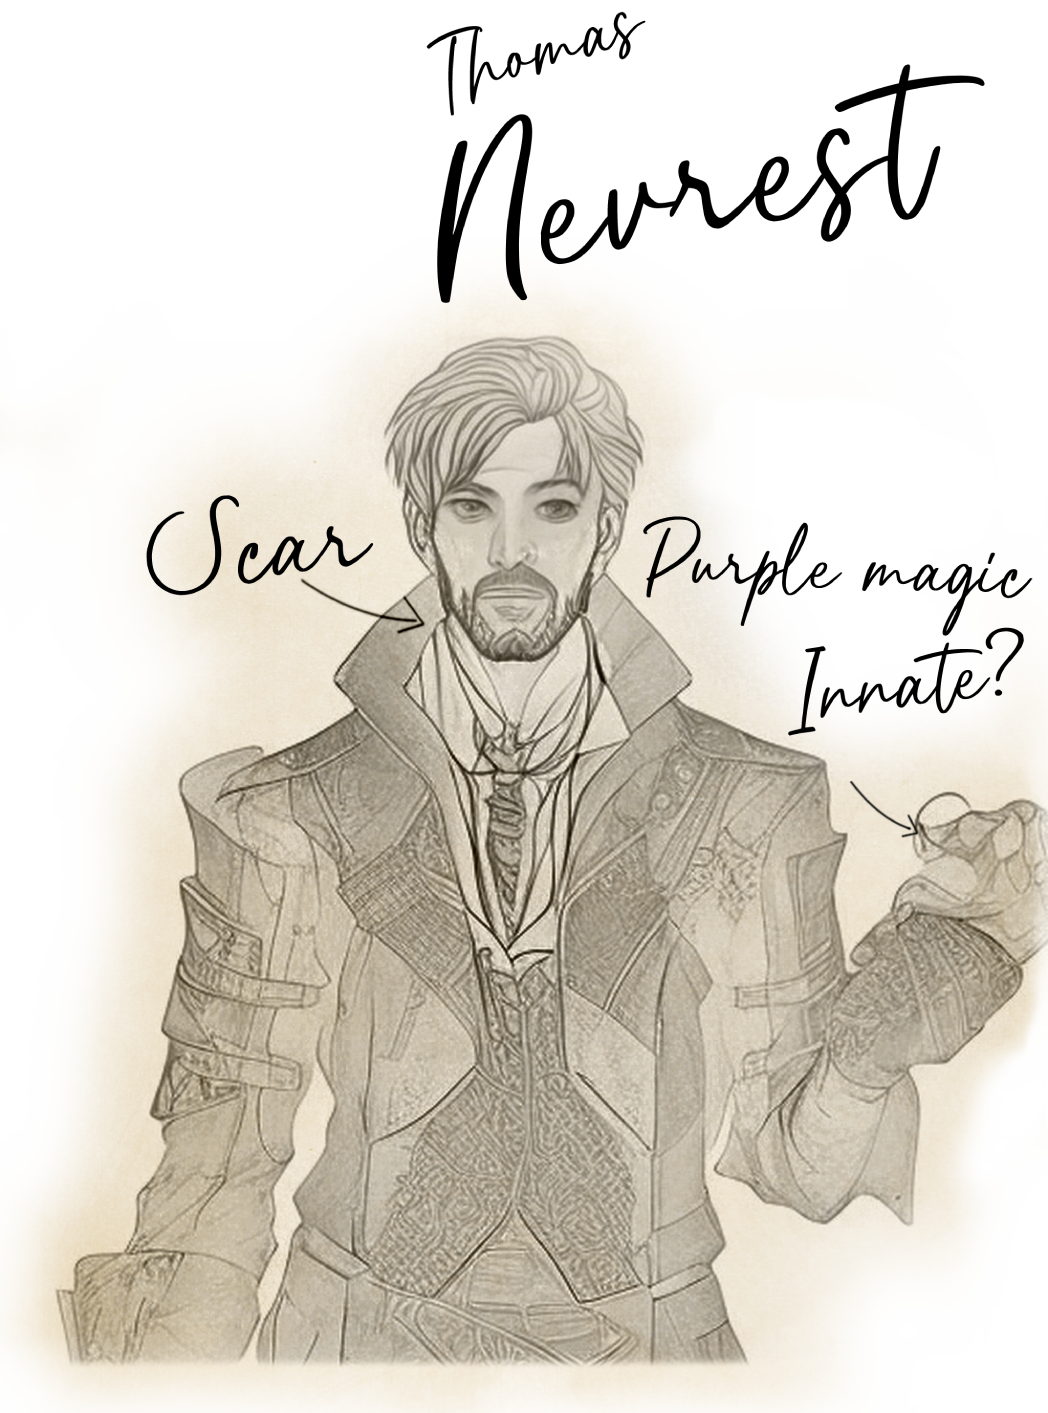
\includegraphics[width=\linewidth-2ex]{images/Nevrest.png}
\begin{DndReadAloud}
    Thomas Nevrest, One of \Name{}'s Companions.
\end{DndReadAloud}
\vfill

\subsection*{The Arena}
I had nothing, no pouch or even you \Master{}. I couldn't cast any spells and I felt what I guess was loneliness, maybe even a kind of nakedness.

We had to fight from time to time, in the arena. There was also an ogre, who they called 'tiny' how ridiculous, guarding the exit door.

We fought some odd figures, stone creatures and all. The group seemed to know them, before they 'turned'. They were very torn fighting them.

\subsection*{The escape}

The following night of some fights, we tried to break into Hargol's, the Orc captain, office. I managed to break in and hide from some frightening monk types. However there was a hidden passageway through the bookcase that we used as our escape.

We found a strange humanoid creature who had an octopus for a head, how bizarre. Nevrest seemed to worship this beast, who was chained up and talking to us telepathically. The head was above water while the rest of his body seemed to be in the water that we weren't supposed to drink.

We freed that wretched creature, it was a pretty big discussion and stirred some commotion. Nevrest was adamant that it was his 'Patron' whatever that means.

After the whole ordeal, we found our belongings and even some other rare item. I even found this book, which I'm now writing in. I've copied you over, \Master{}. I hope you like your new 'cover'.
